 O  filtro de ar escolhido foi o Filtro de partículas de ar de alta performance (HEPA), que possui em sua composição fibra de vidro  e outros materiais, arranjados aleatoriamente, formando uma espécie de teia capaz de filtrar partículas indesejadas. Essas partículas passam e aderem as fribras pelos seguintes mecanismos: \cite{edge}
    
	\begin{enumerate}
	 \item Interceptor: responsável por direcionar as partículas para as fibras.
	 \item Impacto: gera o impacto direto das partículas maiores com a fibra.
	 \item 3. Difusão : partículas com menos de 0,1 mícrons tem maior probabilidade de passar sem serem aderidas pelas fibras, então elas colidem com um gás que as fazem movimentar possibilitando a aderência pela fibra.
	\end{enumerate}
	 
Informações:\cite{filtracom}

	\begin{itemize}
	 \item Possui eficiência mínima de 99,97\% para partículas de 0,3 mícrons;
	 \item Comercializado no Brasil, principalmente, pelas empresas Filtracom e Aeroglass;
	 \item Classes de filtragem: H11, H12, H13, H14 e U15, que atendem as normas europeias EN779, EN1822 e as brasileiras A1 e A3 da ABNT.
	\end{itemize}
	
	\begin{figure}[!htbp]
	 \centering
	  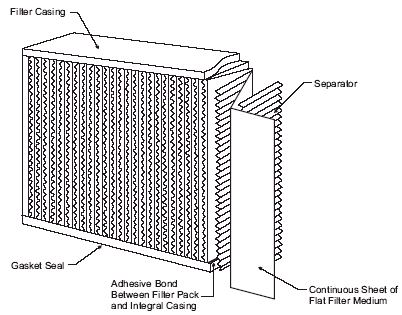
\includegraphics[scale=0.5]{editaveis/figuras/filtro_ar}
	  \caption[Imagem do filtro de ar]{Imagem do filtro de ar\footnotemark}
	  \label{filtro_ar}
	\end{figure}
	\footnotetext{Disponível em: http://www.engineersedge.com/filtration/hepa\_filter.htm }